\section{Systemdesign}

\subsection{Login}
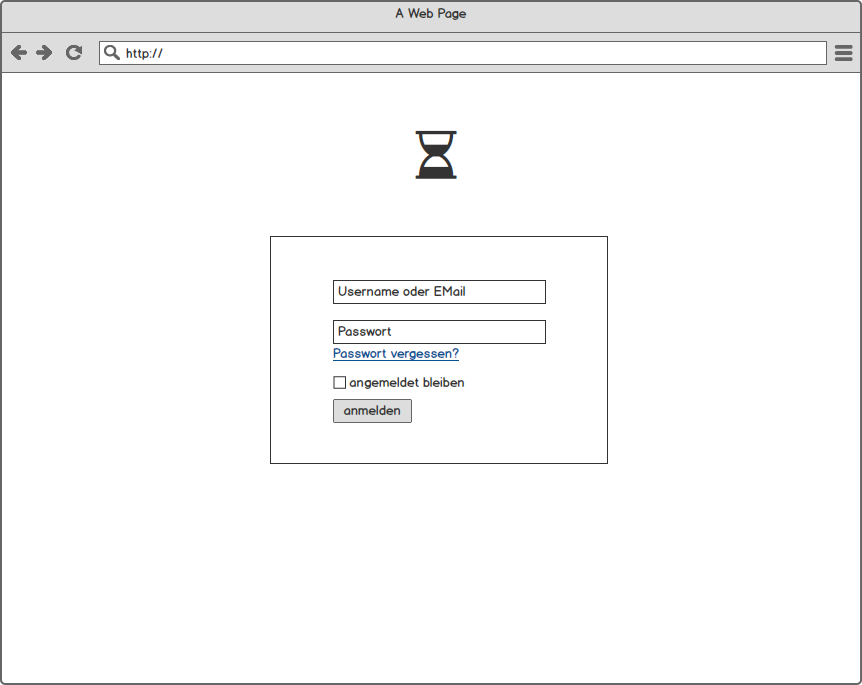
\includegraphics[width=\linewidth]{UI/Login/Login.png}

\newpage
\subsection{Benutzer*}

\textbf{\\Neue Zeiterfassung}\\
\\
Das ist die Hauptseite vom \emph{Benutzer*}, wo er direkt nach einer erfolgreichen Anmeldung oder durch Drücken auf die Schaltfläche "neue Zeiterfassung" landet. \\
Um eine neue Zeiterfassung zu starten, wählt der \emph{Benutzer*} eine Kategorie und eine Tätigkeit aus, anschließend drückt er auf Start Button. Der \emph{Benutzer*} kann die Zeiterfassung über das Stop Button beenden.\\
\\
\\
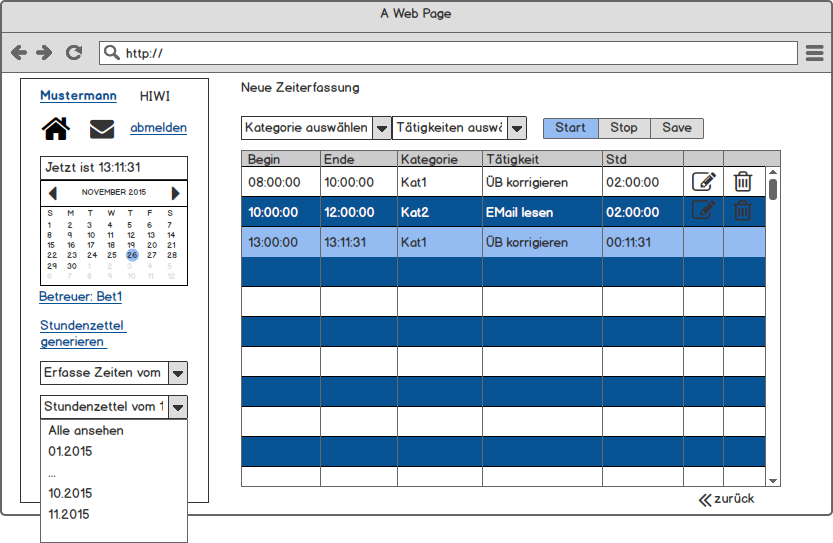
\includegraphics[width=\linewidth]{UI/Benutzer/Zeiterfassung.png}


\newpage
\textbf{\\Erfasste Zeiten bearbeiten}\\
\\
Das ist die Seite fürs Editieren der erfassten Zeiten vom \emph{Benutzer*}.
Man kann entweder direkt von der Seite "Neue Zeiterfassung" über das Edit Button 
\includegraphics[scale=.2]{UI/Button/Edit.png} oder durch auswählen vom Datum auf der Kalenderübersicht auf der linken Seite auf diese Seite landen. Nur die erfassten Zeiten, die noch nicht an den Betreuer abgegeben sind, könnten editiert werden.\\
Der \emph{Benutzer*} klickt in das Textfeld, wo er eine Änderung tätigen will, und ändert die dort eingetragene Daten. Anschließend klickt er auf das Save Button
\includegraphics[scale=.2]{UI/Button/Save.png}, um die Änderungen zu bestätigen.\\
\\
\\
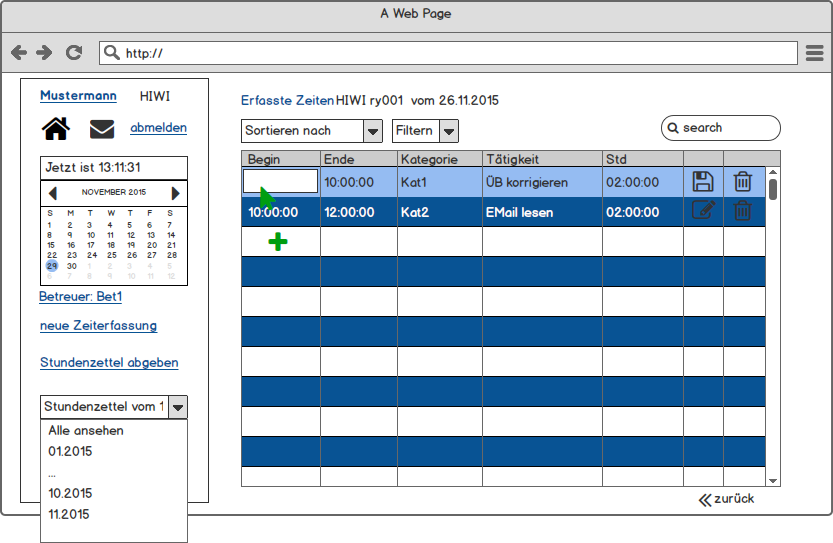
\includegraphics[width=\linewidth]{UI/Benutzer/Editieren.png}






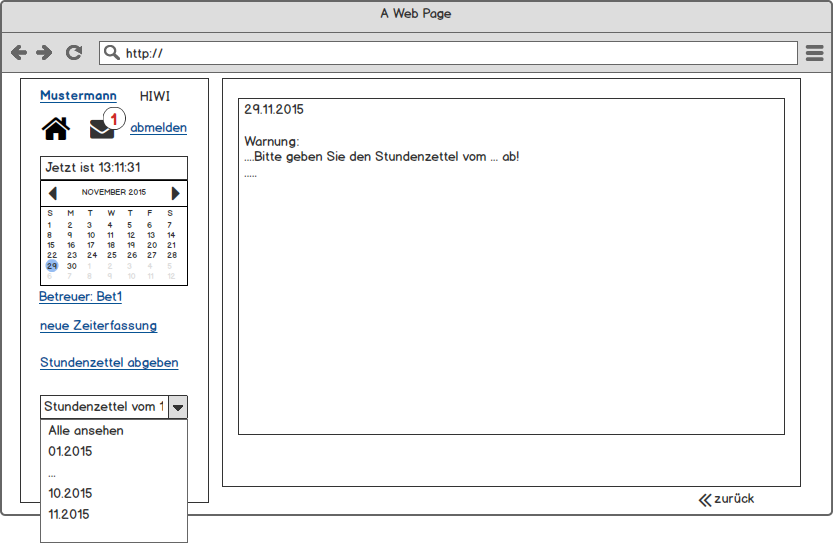
\includegraphics[width=\linewidth]{UI/Benutzer/Nachricht.png}

\subsection{Betreuer}
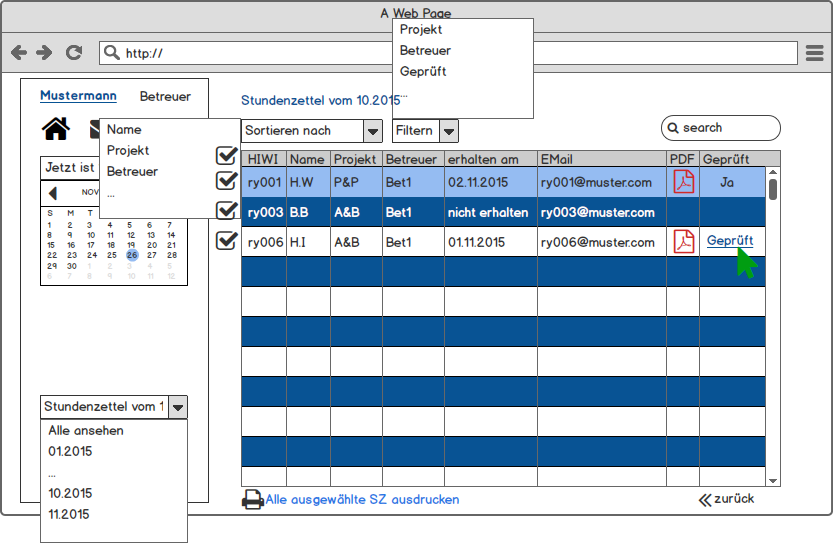
\includegraphics[width=\linewidth]{UI/Betreuer/Hauptseite.png}\\
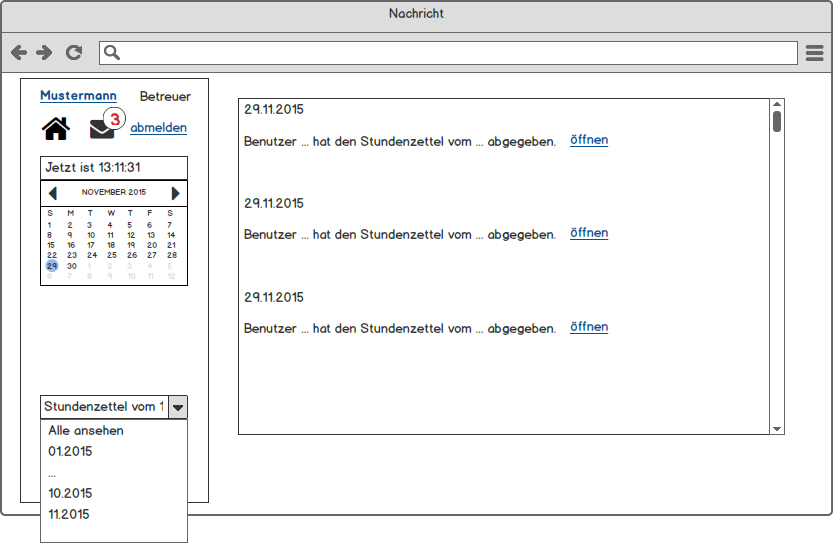
\includegraphics[width=\linewidth]{UI/Betreuer/Nachricht.png}

\subsection{Admin}
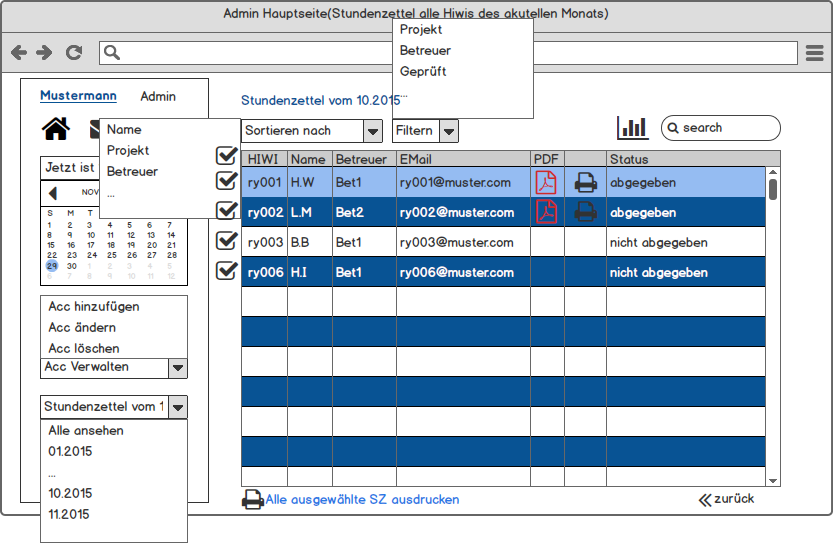
\includegraphics[width=\linewidth]{UI/Admin/Hauptseite.png}
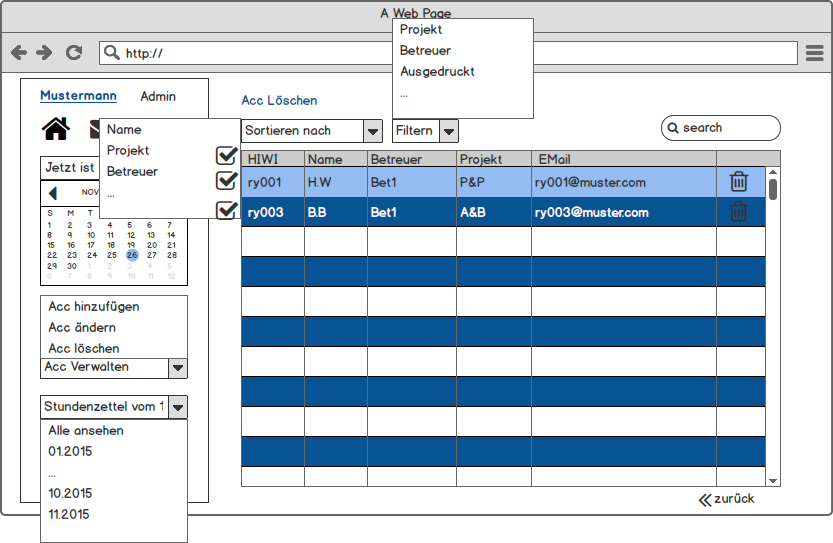
\includegraphics[width=\linewidth]{UI/Admin/Accounts/Ubersicht.png}
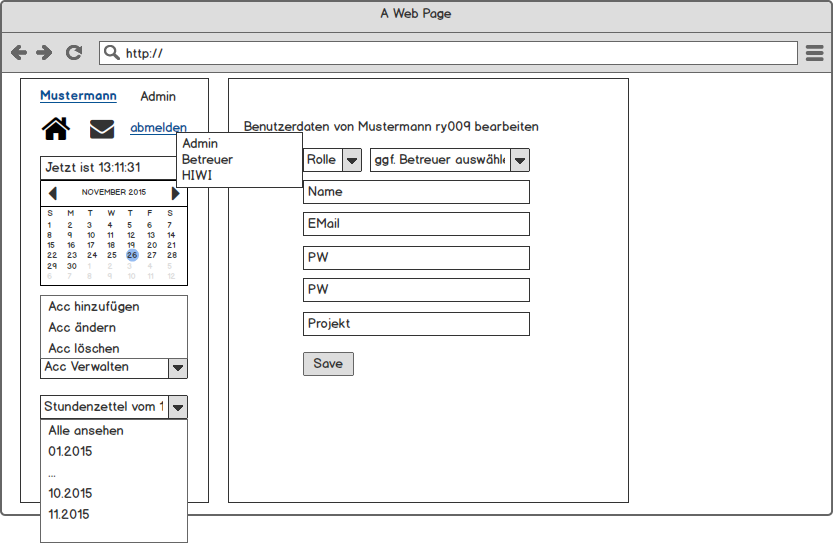
\includegraphics[width=\linewidth]{UI/Admin/Accounts/Bearbeiten.png}
